% This file was created by matlab2tikz.
%
%The latest updates can be retrieved from
%  http://www.mathworks.com/matlabcentral/fileexchange/22022-matlab2tikz-matlab2tikz
%where you can also make suggestions and rate matlab2tikz.
%
\definecolor{mycolor1}{rgb}{0.00000,0.44700,0.74100}%
\definecolor{mycolor2}{rgb}{0.85000,0.32500,0.09800}%
\definecolor{mycolor3}{rgb}{0.92900,0.69400,0.12500}%
%
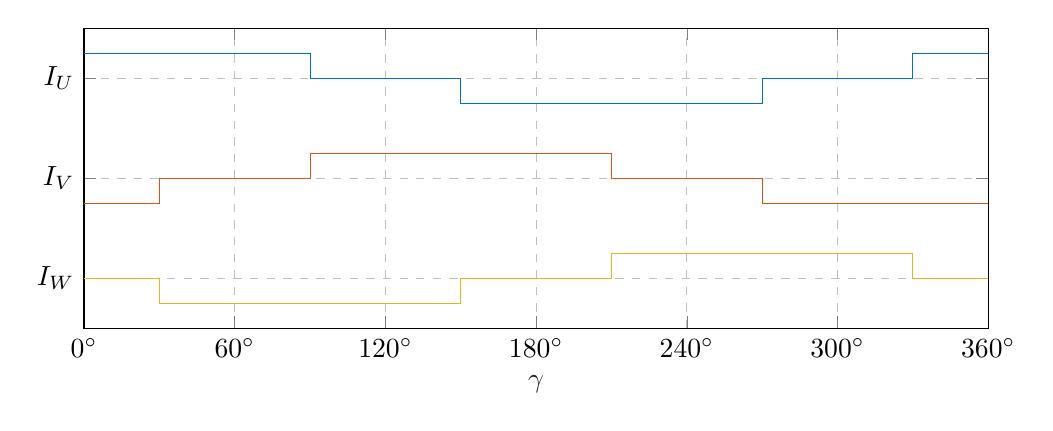
\begin{tikzpicture}

\begin{axis}[%
width=4.521in,
height=1.5in,
at={(0.758in,0.481in)},
scale only axis,
xmin=0,
xmax=360,
xtick={ 0,  60, 120, 180, 240, 300, 360},
xticklabels={{$ 0^{\circ} $},  {$ 60^{\circ} $}, {$ 120^{\circ} $}, {$ 180^{\circ} $}, {$ 240^{\circ} $}, {$ 300^{\circ} $}, {$ 360^{\circ} $}},
xlabel style={font=\color{white!15!black}},
xlabel={$\gamma$},
ymin=-1,
ymax=11,
ytick={1,5,9},
yticklabels={{$ I_{W} $},{$ I_{V} $},{$ I_{U} $}},
axis background/.style={fill=white},
xmajorgrids,
ymajorgrids,
major grid style={dashed}
]
\addplot[const plot, color=mycolor1, forget plot] table[row sep=crcr] {%
0	10\\
30	10\\
60	10\\
90	9\\
120	9\\
150	8\\
180	8\\
210	8\\
240	8\\
270	9\\
300	9\\
330	10\\
360	10\\
};
\addplot[const plot, color=mycolor2, forget plot] table[row sep=crcr] {%
0	4\\
30	5\\
60	5\\
90	6\\
120	6\\
150	6\\
180	6\\
210	5\\
240	5\\
270	4\\
300	4\\
330	4\\
360	4\\
};
\addplot[const plot, color=mycolor3, forget plot] table[row sep=crcr] {%
0	1\\
30	0\\
60	0\\
90	0\\
120	0\\
150	1\\
180	1\\
210	2\\
240	2\\
270	2\\
300	2\\
330	1\\
360	1\\
};
\end{axis}
\end{tikzpicture}%